\subsection{Artefact 1}
    \subsubsection{The Datasets}
    
        The two datasets used to train a cascade classifier for face
        recognition were: 
        \begin{itemize}
            \item Caltech 10,000 Web Faces \cite{fink2007caltech},
                representing the positive values and
            \item The Stanford Background Dataset \cite{hello},
            representing the negative values.
        \end{itemize}
        The first dataset produced by Caltech University
        consists of images of people gathered from the web by
        searching for common given names into  Google images. The
        second dataset consists of 715 outdoor images chosen from
        public datasets.

    \subsection{Training Data preparation}
        \subsubsection{Face Annotation}
            The training data preparation requires item two text files
            containing the directory of each positive and negative
            images and the coordinates of the positive images' faces.
            OpenCV's annotation tool was used to help with annotating
            around 700 faces as can be seen in figure
            \ref{annotationTool}. Few lines from the positive text
            file can be seen in figure \ref{postxt}.

            \begin{figure}[H]
                \centering
                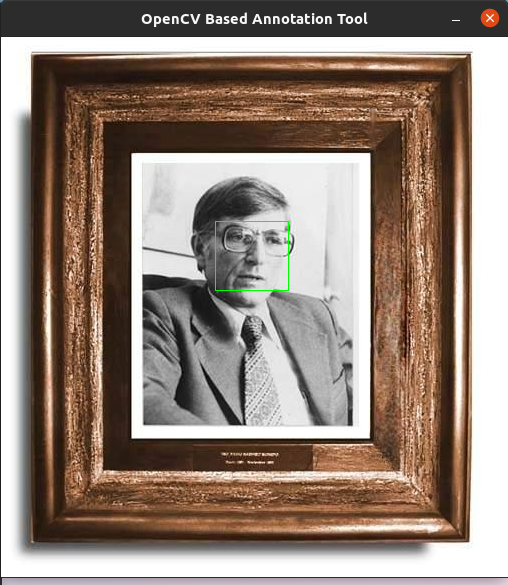
\includegraphics[scale=0.3]{faceAnnotation.png}
                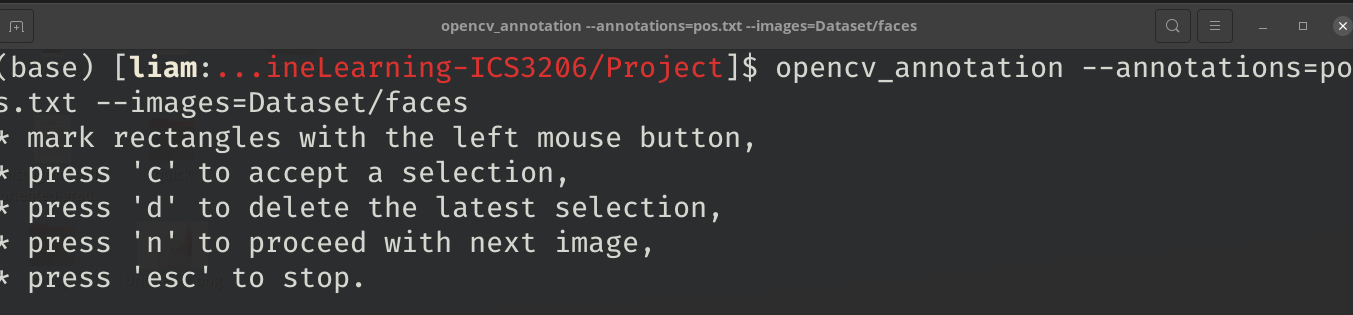
\includegraphics[scale=0.17]{terminalAnnotation.png}
                \caption{OpenCv Annotation Tool in progress}
                \label{annotationTool}
            \end{figure}

            \begin{figure}[H]
                \centering
                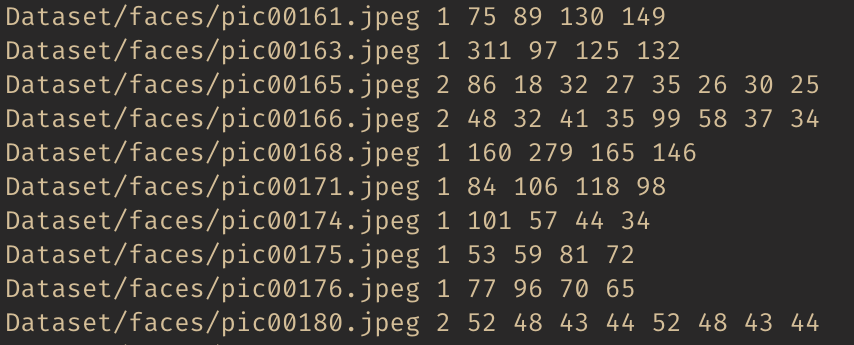
\includegraphics[scale=0.268]{postxt.png}
                \caption{Examples of the Positive Value File}
                \label{postxt}
            \end{figure}

        \subsubsection{Positive Vector File}
            A vector file generated from the positive values' text file is
            also required for cascade training which was generated using
            OpenCV's createSamples program.

    \subsection{Cascade Training}
        The next step is the boosted cascade of weak classifiers based
        on the positive and negative dataset prepared beforehand using
        OpenCV's train cascade function. Several models have been
        generated by changing the parameters' values to meet a good
        result. The evaluation section will show the difference
        between some models compared with the selected xml model that
        have been generated.

            \begin{minted}[
                style=murphy,
            ]{shell}
$opencv_traincascade -data cascade 
-vec pos.vec -bg neg.txt -w 24 -h 24 
-numPos 800 -numNeg 425 -numStages 15
-precalcValBufSize 3000 -precalcIdxBufSize 
3000 -maxFalseAlarmRate 0.4
            \end{minted}

\subsection{Artefact 2}

    Artefact 2 The two downloaded models
    haarcascade\_frontalface\_default.xml, haarcascade\_eye.xml for
    the frontal face and eyes, respectively,  are tested using
    OpenCV's \textbf{cascadeClassifier} function. Check for the
    results and comparisons in the evaluation section.
    
\section{Results}